\documentclass[a4paper,12pt]{book}

%%%%%%%%%%%%%%%%%%%%%
% Front page
%%%%%%%%%%%%%%%%%%%%%
%%%%%%%%%%%%%%%%%%%%%
% Front page
%%%%%%%%%%%%%%%%%%%%%
\makeatletter
\def\thickhrulefill{\leavevmode \leaders \hrule height 1pt\hfill \kern \z@}
\def\maketitle{\null \thispagestyle{empty} \vskip 1cm
  \begin{flushright}\normalfont\Large\@author\\\end{flushright}
  \vfil
  \hrule height 2pt
  \par
  \begin{center}\huge \strut \@title \par \end{center}
  \hrule height 2pt
  \begin{center} \par \end{center}
  \begin{center}
\includegraphics[width=0.60\textwidth]{./hs}\end{center}
  \par \vfil \vfil \null
  }
\makeatother
%%%%%%%%%%%%%%%%%%%%%
% Libraries
%%%%%%%%%%%%%%%%%%%%%
%%%%%%%%%%%%%%%%%%%%%
% Libraries
%%%%%%%%%%%%%%%%%%%%%
%\usepackage[T1]{fontenc}
%\usepackage[dvips]{graphicx}
%\usepackage{hyperref}
\usepackage[pdftex]{graphicx} %PDF Graphik
\usepackage[pdftex]{hyperref} %PDF Referenzen
\usepackage{times}
%\usepackage{float}
%\usepackage{floatflt}
\usepackage{amsmath}
\usepackage{amssymb}
\usepackage{amsthm}
%\usepackage[ngerman,english]{babel}
\usepackage[right]{eurosym}
\usepackage{color}
\usepackage{ulem}
\usepackage{longtable}
\usepackage{multirow}
\usepackage{ltxtable}
\usepackage{ragged2e, tabularx}
\newcolumntype{Y}{>{\RaggedRight\arraybackslash}X}
\usepackage{cancel}
\usepackage{wrapfig}
%%%%%%%%%%%%%%%%%%%%%
% Macros
%%%%%%%%%%%%%%%%%%%%%
%%%%%%%%%%%%%%%%%%%%%
% Macros
%%%%%%%%%%%%%%%%%%%%%
\newcommand{\asregkopf}[2]{
\begin{center}
\begin{tabularx}{\textwidth}{Xr}
  %{#1} & \begin{flushright}[Reset value: {#2}]\end{flushright}
  {#1} & [Reset value: {#2}]
\end{tabularx}
\end{center}
}

\newcommand{\asregtwoxsixteen}[4]{
\begin{center}
\begin{tabularx}{\textwidth}{|X|X|X|X|X|X|X|X|X|X|X|X|X|X|X|X|}
  \hline
  31 & 30 & 29 & 28 & 27 & 26 & 25 & 24 & 23 & 22 & 21 & 20 & 19 & 18 & 17 & 16  \\
  \hline
  #1 \\
  \hline
  #2 \\
  \hline
  \hline
  15 & 14 & 13 & 12 & 11 & 10 & 09 & 08 & 07 & 06 & 05 & 04 & 03 & 02 & 01 & 00 \\
  \hline
  #3 \\
  \hline
  #4 \\
  \hline
\end{tabularx}
\end{center}
}

\newcommand{\asregfour}[2]{
\begin{center}
\begin{tabularx}{\textwidth}{|X|X|X|X|}
  \hline
  3 & 2 & 1 & 0 \\
  \hline
  #1 \\
  \hline
  #2 \\
  \hline
\end{tabularx}
\end{center}
}

\newcommand{\asregeight}[2]{
\begin{center}
\begin{tabularx}{\textwidth}{|X|X|X|X|X|X|X|X|}
  \hline
  7 & 6 & 5 & 4 & 3 & 2 & 1 & 0 \\
  \hline
  #1 \\
  \hline
  #2 \\
  \hline
\end{tabularx}
\end{center}
}

\newcommand{\asregdesc}[1]{
\begin{center}
\begin{tabularx}{\textwidth}{|l|l|l|X|}
  \hline
  \textbf{Field} & \textbf{Bits} & \textbf{Type} & \textbf{Description} \\
  \hline
  #1 \\
  \hline
\end{tabularx}
\end{center}
}
\newcommand{\chipname}{\textbf{HS-Weingarten Phase ASIC} }
\newcommand{\designUnita}{\textbf{ccreg} }
\newcommand{\designUnitb}{\textbf{ucreg} }
\newcommand{\ioa}{\textbf{S0\_i} }
\newcommand{\iob}{\textbf{S1\_i} }
\newcommand{\ioc}{\textbf{SP\_i} }
\newcommand{\iod}{\textbf{SX\_i} }
\newcommand{\ioe}{\textbf{ena\_i} }
\newcommand{\iof}{\textbf{adr\_i} }
\newcommand{\iog}{\textbf{di\_i(3:0)} }
\newcommand{\insiga}{\textbf{rx\_ready\_s} }
\newcommand{\insigb}{\textbf{phase\_ready\_s} }
\newcommand{\supplya}{\textbf{VDD\_MAIN} }
\newcommand{\ChipClka}{\textbf{clk\_i} }
\newcommand{\ChipClkaspeed}{\textbf{100MHz} }
\newcommand{\ChipRsta}{\textbf{rst\_n\_i} }
\newcommand{\ChipIOa}{\textbf{tx\_o} }
\newcommand{\ChipIOb}{\textbf{rx\_i} }


\usepackage{tabularx} % in the preamble

\begin{document}
\title{S4-VHDL Specifications}
\author{Nils Schlegel, 32067\\Tara Jaishi, 32289}
\date{\today}
\maketitle %\tableofcontents

\setcounter{chapter}{0}


1 Product: IC{\_}4 \\
\begin{center}
\begin{tabularx}{\textwidth}{llX}
History \\
\cline{1-3}
Target Spec. & Current version: 0.1, 2020-11-9 \\
& Previous version: - \\
\cline{1-3}
& 06.11.2020 & General description added \\
& 06.11.2020 & Blockdiagram added \\
& 06.11.2020 & Functional description added \\
\end{tabularx} \\
\end{center}
1.1 General-description \\
IC{\_}4 is a single chip based application containing processing capabilities to detect and keep track of the amount of people in one room. It is part of a system solution to fullfill the covid-19-restrictions and  regulate the amount of people in an area. This solution is only meant for a chamber with only one doorway available to enter or to exit. \\
The IC{\_}4 is designed on a PGA prototype-board Max1000 with 10M16SAU169C8G Device on board.

\begin{center}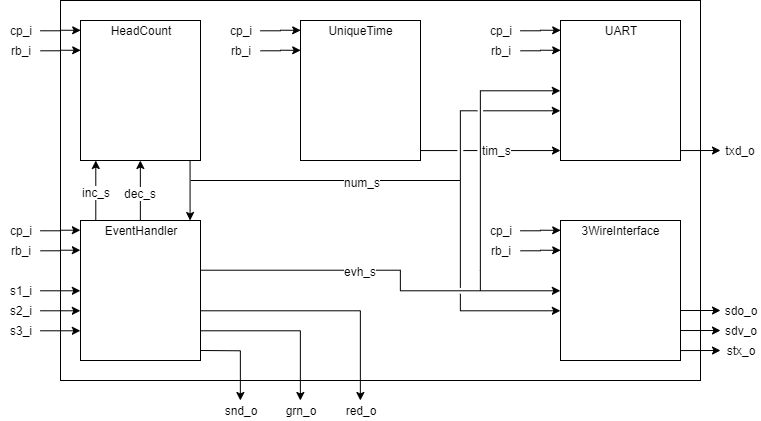
\includegraphics[width=1\textwidth]{./top}\end{center}

\begin{center}
\begin{tabular}{lll}
rb{\_}i & reset & reset, active low \\
cp{\_}i & system clock & e.g. 10 MHz \\
s1{\_}i & light{\_}curtain s1 & log1: something passes \\
s2{\_}i & light{\_}curtain s2& log1: something passes \\
s3{\_}i & light{\_}curtain s3 & log1: something passes \\
%rb{\_}o & reset led & emits light, when reset is !active \\
grn{\_}o & LED, access garanted & Green LED, go ahead \\
red{\_}o & LED, stop, no entry & Red LED, stop, access denied \\
sdo{\_}o & serial data out & drives S3 or MC \\
sdv{\_}o & serial data valid & drives S3 or MC \\
stx{\_}o & serial transfer active & drives S3 or MC \\
txd{\_}o & serial out & to RS-232-driver,9k6,8N2,ASCII,to PC \\
snd{\_}o & sound signal & acoustic signal, to loudspeaker \\
\\
inc{\_}s & increment & increments head count when triggered \\
dec{\_}s & decrement & decrements head count when triggered \\
num{\_}s & number & contains the head count number \\
evh{\_}s & event & contains the current event \\
\end{tabular}
\end{center}

1.2 Functional-description \\
\\
HeadCount \\
Stores the current number of people in the room. It increments or decrements the number if needed.
\\
\\
EventHandler \\
It receives the signals from the light curtains and detects which event is triggered. Depending on the event it will play a sound, turn on a LED and create an output signal.
\\
\\
UniqueTime \\
This element is only counting the clock-cycles, to generate a unique timestamp.
\\
\\
UART \\
The connection to the RS232 is done by the UART. It takes the unique timestamp from the UART as well as the head count from the HeadCount and event type from the EventHandler, when a signal from the EventHandler is received.
\\
\\
3WireInterface \\
The IC{\_}3 can be connected by using the 3WireInterface. When it receives a signal from the EventHandler it should pass the head count and event type to the IC{\_}3.

\end{document}
